% This is LLNCS.DEM the demonstration file of
% the LaTeX macro package from Springer-Verlag
% for Lecture Notes in Computer Science,
% version 2.2 for LaTeX2e
%
%\documentclass[12pt]{llncs}
%\documentclass[envcountsame,oribibl,11pt]{llncs}
\RequirePackage{amsmath}
\documentclass[runningheads,a4paper]{llncs}
%\documentclass[runningheads,a4paper]{llncs}
%\usepackage[hmargin=1in,vmargin=1.25in]{geometry} 

\usepackage{amsmath, amssymb}
\usepackage{algorithm,algorithmic}
\usepackage{makeidx}  % allows for indexgeneration
\usepackage{graphicx,epsfig,color}
\usepackage{boxedminipage}
\usepackage{multicol} 
\usepackage{enumerate}
\usepackage{diagbox}
\usepackage{float}
\usepackage[table]{xcolor}
\usepackage{multirow}
\usepackage{longtable}
%\usepackage{titlesec}

\setcounter{secnumdepth}{5}
% To use "Arial" font, use the following 2 lines
%\renewcommand{\rmdefault}{phv} % Arial
%\renewcommand{\sfdefault}{phv} % Arial

% The following statement specifies the amount of space between
% paragraphs. Other reasonable specifications are \bigskipamount and \medskipamount.
%\setlength{\parskip}{\smallskipamount}

% The following statement controls the line spacing.  
%\renewcommand{\baselinestretch}{1.0}

% TRACK CHANGE
% ------- Bar -------
%\begin{changebar}
% The proposed scheme
%\end{changebar}
% ------- Highlight -------
%\hl{scheme} 
% ------- Strikeout -------
%\st{framework}
%\usepackage{soul}
%\sethlcolor{green}
%\setstcolor{red}
%\usepackage[color]{changebar}
%\cbcolor{blue}

\begin{document}

%\bibliographystyle{abbrv}	% [1] A. Author. Article name, ...
\bibliographystyle{acm}	% [1] AUTHOR, A. Article name. ...
%\bibliographystyle{alpha}	% [Las98] Firstname Lastname. Article title. ... [alphabetical order]
%\bibliographystyle{apalike} 	% [Author, 1990]
%\bibliographystyle{amsplain}	% [1] Firstname Lastname, Italicized Article Name, ... 
								%        [authors in alpha order, underscore for repeated author]
%\bibliographystyle{ieeetr}	% [1] F. Writer. "Article name", ... [in order of reference]
%\bibliographystyle{plain}	% [1] Firstname Lastname. ...
%\bibliographystyle{siam}	% [1] A. AUTHOR, Italicized Article Name, ...
%\bibliographystyle{unsrt}	% [1] Firstname Lastname. Article name. ... [in order of reference]

%
\frontmatter          % for the preliminaries
%
\pagestyle{headings}  % switches on printing of running heads
\addtocmark{Title of The Paper} % additional mark in the TOC
%
\mainmatter              % start of the contributions
%
\title{A Survey on Trust in Autonomous Systems \\ 
}
%
\titlerunning{A survey on Trust}  % abbreviated title (for running head)
%                                     also used for the TOC unless
%                                     \toctitle is used
%
\author{\large Shervin Shahrdar and Mehrdad Nojoumian   %\inst{1} \thanks{Research supported by X.} 
%and Name-2 %\inst{2} \thanks{Research supported by X.}
}

\authorrunning{ Shervin Shahrdar  \& Mehrdad Nojoumian
}   % abbreviated author list (for running head)

\institute{
Department of Computer \& Electrical Engineering and Computer Science \\ Florida Atlantic University, Boca Raton, FL, USA \\
\email{sshahrda@fau.edu}, \url{www.shervinshahrdar.com} \\
\email{mnojoumian@fau.edu}, \url{http://faculty.eng.fau.edu/nojoumian/}
}

\maketitle
\begin{abstract}

\noindent As a result of the exponential growth in technology and computing in the past couple of decades, autonomous systems are becoming more relevant in our daily lives. As these autonomous systems evolve and become more complex, the concept of trust in such systems becomes a major challenge that affects the performance, and reliability of such systems. Many prior studies have indicated that currently, humans have a very low trust-level in the fully autonomous robots. Similarly, trust between autonomous systems plays a major role in their performance. In this meta-analysis, we will explore various research and trust models in order to show why trust management is a very challenging aspect of future AI technologies.

\vspace{10pt}
\textbf{Keywords:} Trust Function, Reputation Systems, Autonomous Systems, Multi-Agent Systems
\end{abstract}

%\addtolength{\parskip}{1.6ex}
%\parindent 0pt

%-------
\section{Introduction} 
\label{ShervinTrustSurvey_introduction}
The rapid growth in technology has resulted in the automation of many day to day tasks that humans had to perform themselves just decades ago. From ATMs (Automated Telling machines) to industrial robots used in factories, automation continues to aid humans with repetitive, difficult, and monotonous tasks. This technological advancement introduces newer and more complex robotic concepts, and automated systems in different areas of our lives including our homes, daily commute, workspace, military, and many other areas every day.

As these automated systems evolve, their levels of complexity increase overtime, and their involvement in various aspects of human life introduces the concept of human-robot trust. Studies have indicated that one of the most important challenges for successful integration of advanced autonomous systems and AI technology in human civilization, will be the management and the development of this mutual trust \cite{beer2014toward}.

In this paper, we will provide a step by step, comprehensive analysis and explore various concepts and related studies, as well as experimental techniques proposed by researchers in this field, in order to understand how the human-robot trust management works, and how we can improve it. Additionally, we will explore the trust between autonomous systems (Agents) in section 3.

\section{Definitions}
\subsection{What is an Autonomous System?}
First, an autonomous system needs to be defined. This definition keeps changing everyday as the related technology grows exponentially \cite{schaefer2013perception}.

Merriam Webster dictionary defines `autonomy' as  ``The quality or state of being self-governing; especially: the right of self-government''. The concept of Autonomy has existed for thousands of years, in many different areas including philosophy, sociology, politics, and technology. In fact, the second part of the term Autonomous, \textsl{nomos}, means `law' in  Greek. An autonomous entity ``creates its own laws''. \cite{MerriamWebsterAtn}. 

We need to narrow down this definition, as this it is very broad and applies to many different areas and concepts. Perhaps the term that we are looking for is `autonomous robots'. Autonomous robots are defined as, ``intelligent machines capable of performing tasks in the world by themselves, without explicit human control.'' \cite{Bekey:2005:ARB:1088950}

\begin{figure}
	\centering
		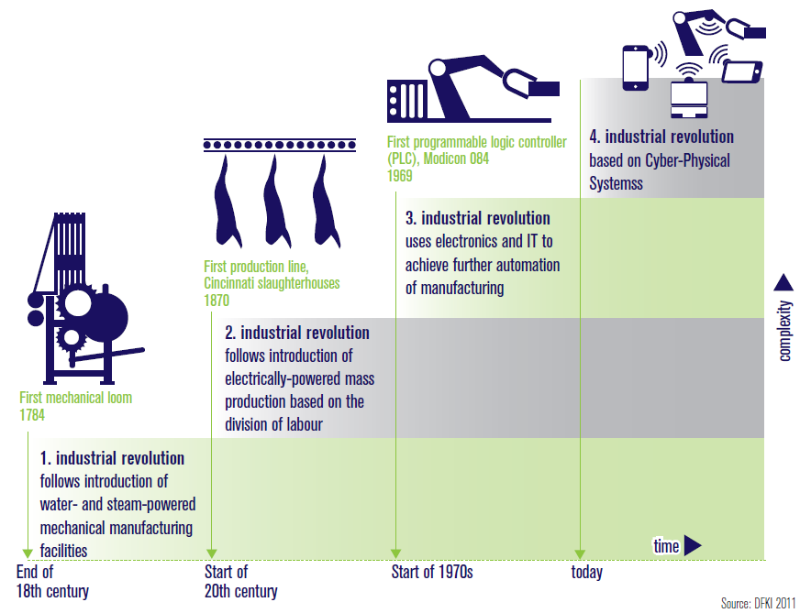
\includegraphics[width=\textwidth]{Figures/EvolutionOfAutomation.png}
	\caption{Evolution of Automation \cite{CyberSecurityInIndustry}}
	\label{Trust_Function}
\end{figure}
Although automation was introduced to human civilization many years ago, and widely used after industrial revolution in early 1800s \cite{IndustrialRevolution}, Autonomous systems, and Industrial Robots are relatively new terms that were introduced merely decades ago, and their definitions are evolving everyday, as technology advances. In this paper, our main focus will be on Autonomous Robots and Autonomous Agents which are a highly advanced form of automated machines that have a high degree of self-awareness, and are capable of independently performing tasks which were previously done by humans.

\subsection{What is Trust?}
`trust' is a concept that has many different definitions in various contexts such as psychology, sociology, and Economics. Currently, there is no uniform definition of `trust' in the context of psychology, or other areas \cite{adams2003trust}. Prior research indicates that there are over 300 definitions in various research areas, and in the context of Human-Robot relationships, which is our focus in this paper, there are more than 30 definitions. These definitions include `human interpersonal trust', `automation trust', `trust in software agents'', and many others \cite{schaefer2013perception}. 

Although there are complex definitions of trust documented based on the area of the research,  we shall focus on the simplest, domain-agnostic definition. A very simple, generic definition of `trust' would be: ``A firm belief in the reliability, truth, or ability of someone or something'' \cite{oxfordDicTrust}. If we consider this simple definition, then, in our research context, the definition of trust would be: ``A strong human belief in the reliability, truth, or ability of an autonomous system''. The `Autonomous system' in this case could be any kind of a self aware machine that has a high degree of autonomy. Some concrete examples would be human trust in self driving cars (SDC), autonomous planes, battlefield robots, rescue robots, autonomous software agents, and so on.

\section{Review of Literature: Trust in Autonomous Systems}
In this section, we will review, and categorize previous studies that are in the domain of human-robot trust relationship.

\subsection{Trust Between Humans and Autonomous Systems}

\subsubsection{Human-Robots}
As previously stated, many studies have shown that currently, the level of trust between humans and autonomous systems is very low. That means in serious situations, humans tend to not let fully autonomous systems take control. A study that explores the low level of human-robot trust, is done by Daniel Stormont (2008) \cite{stormont2008analyzing}. In this study, the factors that affect the trust between humans and robotic systems are analyzed. The study concluded that it is not just `trust' that determines the usability, but `confidence' also plays a significant role. One of the reasons the level of confidence in autonomous systems is very low is due to their low level of reliability. As cited in this paper, ``A 2004 study of commercially available ruggedized robots operating in
field conditions showed a mean-time-between-failures
(MTBF) of 12.26 hours and an availability rate of 37\%''\cite{carlson2004investigation}. This means, that if the robotic systems reduce their failure rate, their reliability will increase, thus, the human confidence and trust in them will increase. Of course this study was done in 2004. It is clear that due to recent advancements in robotic systems, the MTBF should be definitely less than 37\%. For example, when the first fatal car accident was reported for Tesla self driving cars, it became a topic of discussion in the media. Although these accidents are rare, companies like Tesla and Google learn the nature of the accident, and work on reducing the failure rate in the future models. \cite{TeslaFatalAccident}

In his research, Mr.Stormont (2008) also believes that another factor affecting the trust between humans and fully autonomous systems would be their unpredictability. It is known that in various hazardous circumstances such as battlefields and rescue missions, the unpredictability of robots becomes a critical problem for human supervisors. It has been argued that the autonomous nature of robots, and their decisions making could be a positive trait, since they could react faster to certain dangers compared to humans, but the problem arises when life and death of humans will depend on the choices of a robot; Questions such as ``should life and death decisions be made
by an autonomous system?'' will emerge. In the 2008 study, a simulation of robots assisting firefighters in a hazardous fire situation was discussed. It was concluded that even though firefighters did not initially trust these helper robots, as the mission went on, and they got tired, their reliance and trust in the robots increased, as they helped them extinguish the fire. 
\begin{figure}
	\centering
		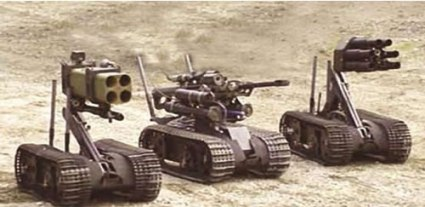
\includegraphics[scale=0.6]{Figures/3robots.jpg}
	\caption{Example of autonomous and semi-autonomous robots used in military \cite{autonomousArmedRobots}}
	\label{MilitaryRobots}
\end{figure}

Another study conducted by Mr. Babak Esfandiari and his colleague, Mr. Sanjay Chandrasekharan \cite{esfandiari2001agents} thoroughly examined and proposed ``simple
mechanisms for trust acquisition based on a very basic and general definition of trust.'' According this this study, the majority of views on the definition of trust are divided into two groups: Cognitive views, and mathematical views. Mr. Esfandiari argues that both of these views have something in common: both of them see `trust' as a variable, that also has a threshold for an action. This action is called cooperation. The mathematical definition of `trust' provided by this study is: ``Trust is a function T between any two agents of a set A of agents''. These agents can be humans, or robots, or autonomous systems, and so one. This study also provides a concept called `Trust Acquisition'. Given an example of previously defined mathematical function: T(Alice, Bob) (Trust between Alice and Bob), Trust Acquisition is described as ``the process or mechanism that allows the calculation and update of T. In our
definition, acquisition is not necessarily an 'increase' of T.''. This study provides various methods of Trust Acquisition:
\begin{enumerate}
	\item Trust Acquisition by Observation
	
	Mr. Esfandiari argues that Trust Acquisition can be obtained by performing `Bayesian Learning'. This means that agents observe, and consider that past actions of other agents, and decide whether to perform an action or not. This paper provides an example of two agents, RoboCop robots John and Mary. John has the ball, and is deciding whether or not pass the ball to Mary, or just shoot the ball himself. If John is able to review the past performances of Mary, and compares them with his own performance, and performs a statistical analysis, he will be able to make a decision.
	\item Trust Acquisition by Interaction
	
	In Trust Acquisition by Interactions protocol, agent 1 asks a bunch of pre-determined questions from agent 2. Agent 1 already knows the answer, thus, the trust will be acquired based on the the number of correct answers provided by agent 2.
	\item Trust Acquisition Using Institutions
	This study provides an example of humans trusting police officers wearing uniforms. If a person sees another person equipped with a gun who is wearing a uniform, he will automatically trust that person, because the trust is already established by the institution. However, if he sees a person not wearing a uniform and carrying a gun, he needs to make more calculations to trust this person.
	
\end{enumerate}


In a 2011 paper, Peter A. Hancock et al. provided a comprehensive analysis of factors affecting trust in ``Human-Robot Interaction (HRI)'' \cite{hancock2011meta}. This study categorizes factors that affect the trust in HRI into three different categories: human related, Robot related, and environmental variables, and each category has sub categories. Human related factors include training, expertise, situational awareness, demographics etc. Similarly, robot-related factors are behavior, dependability, reliability, level of automation, failure rates, false alarms, and transparency, and attribute based factors such as location, personality, adaptability, robot type, and Anthropomorphism (having human traits). Environmental factors include team work, culture, communication, shared mental models, task type, task complexity, multi-tasking, physical environment. This paper discovered that robot performance has the biggest impact on trust in the context of HRI, and tweaking the robot performance has a direct impact on trust. For example, if an autonomous robot improves its performance, the value of trust will increase.

\begin{figure}
	\centering
		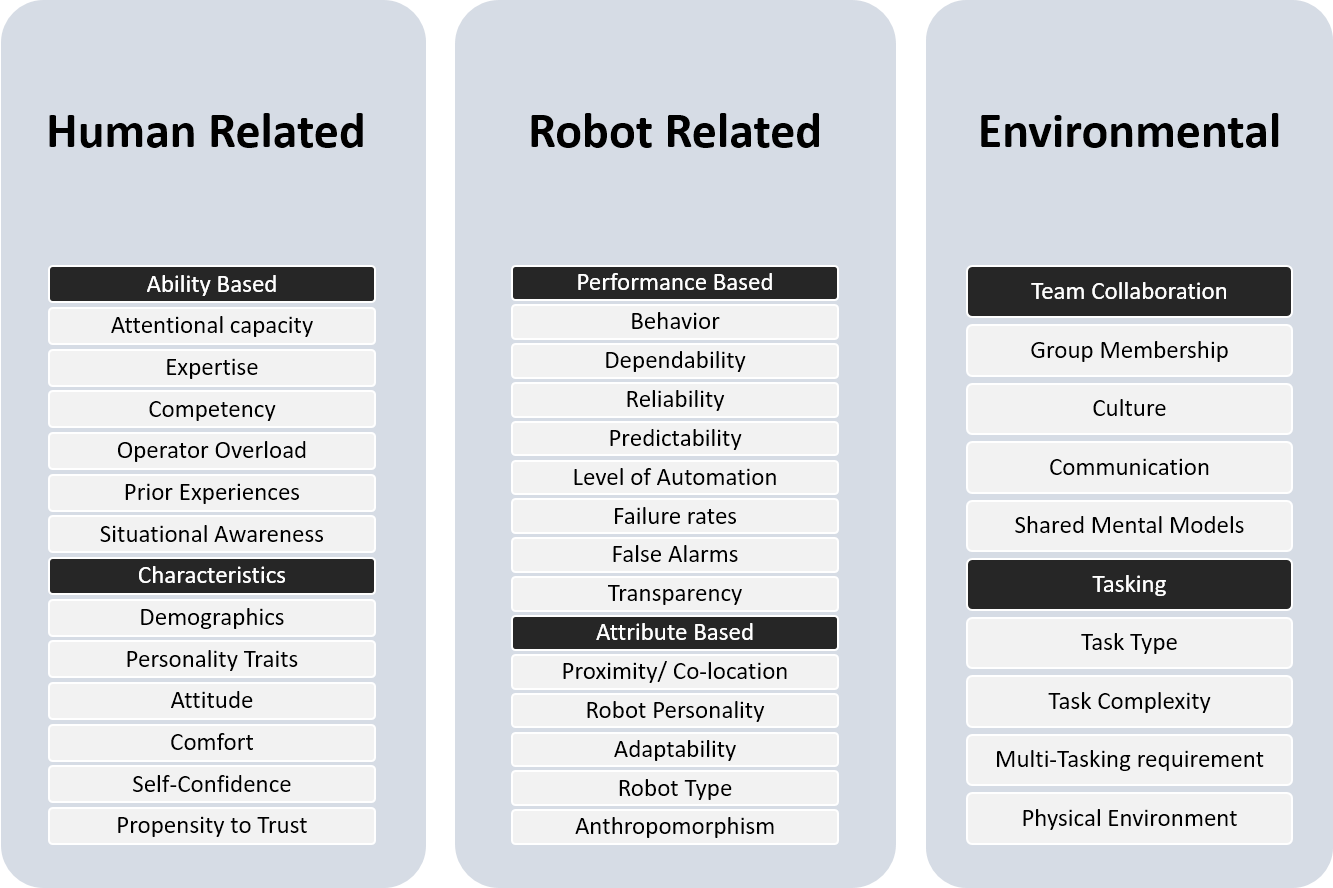
\includegraphics[width=\textwidth]{Figures/TrustFactors.png}
	\caption{Trust factors identified by Hancock \cite{hancock2011meta}}
\end{figure}

\newpage

Jacques Penders and his co-workers investigated HRI in `no-visibility' conditions \cite{penders2013enhancing}. No visibility condition in this context means that the human user might be visually impaired, or completely blind, therefore, they would have to completely trust the robot. This study also takes a look at the attributes in the design of robots that affect the ethical behavior of them. Additionally, this study analyzes the interaction of visually impaired person and their guide dog, and examines the variables that could be implemented in the design and behavior of robots to improve the human confidence in them. These variables include human dominance, cooperation overtime, and accountability.

In \cite{merritt2008not}, Stephanie Merritt at the University of Missouri examined the importance of taking differences in human behavior into consideration in the context of HRI. Ms. Merritt completed this empirical study by providing an experiment related to  X-ray screening. Subjects were asked to use a simulation software to detect dangerous items such as weapons, in different luggage. They given the options of scanning the x-ray image manually, and flagging it if they spot a suspicious item, or have a fictional autonomous system called  Automatic Weapons Detector(AWD) scan the image, and report any issues. This study concluded that the individual differences in subjects affects the value of trust in autonomous systems, even if the characteristics of the autonomous system is `constant'. Thus, this study suggests that future researchers in the field of HRI and trust should take human characteristics into consideration.

Raja Parasuraman and Christopher Miller investigated the concept of trust and etiquette in the domain of HRI \cite{parasuraman2004trust}. Given the fact that in many human-to-human social interaction scenarios, respect and etiquette highly influence the level of trust. Mr. Parasuraman and Mr. Miller argued that they also influence the perception of autonomous robots in humans. In this paper, etiquette is described as: ``the set of prescribed and proscribed behaviors
that permits meaning and intent to be ascribed to
actions.''. This study also provides an experiment related to the role of etiquette in HRI. In order to assess the influence of etiquette, test subjects used a flight simulator software called Multi-Attribute Task (MAT), and communicated with the autonomous system using different communication styles such as interrupting the user, being impatient, etc. The empirical evidence obtained by this experiment indicated that etiquette definitely influences the human trust, and reliability of autonomous robots.

A research conducted by Ms. Rosemarie Yagoda and her research partner, Mr. Douglas Gillan, provided a mechanism for measuring the value of trust in the context of HRI \cite{yagoda2012you}. This measurement is based on multiple factors, including team configuration, team processes, context, task, and system. This trust scale measuring mechanism is based on two studies in this research. In this first study, subject matter experts, and previous studies were used to construct a `content validity assessment'. The second study examines the trust scales obtained from the first study. The results of these two studies were combined to create the `HRI Trust Measuring Tool'.

In a 2014 paper, Yue Wang and partners investigated the human-robot trust in the context of underwater semi-autonomous robots \cite{wang2014human}. In order for the underwater robot to have a good performance, the person who is operating the robot needs to trust its autonomous capabilities. This study proposed a trust model that mainly deals with recording the robot's past performance, the human performance, and the fault rates of humans and robots. The semi-autonomous robot `YSI EcoMapper AUV' was investigated in this study specifically. Furthermore, MATLAB simulations indicate the effectiveness of this trust model.

\subsubsection{Human-Self Driving Cars (SDCs)}
Autonomous driving has been advancing exponentially in the recent years due to technological advancements in AI, mechanics and advanced sensor systems. Car manufacturers such as Google, Tesla, Mercedes-Benz, Ford, and many others have already created commercially available semi-autonomous cars, and fully autonomous prototypes, and they expect mass production of self driving cars (SDCs) in the early 2020s \cite{driverlessFutureForcast}. One major challenge in popularizing SDS in the US and the world would be the high level of distrust of average consumers in fully automated vehicles.

Daniel Howard at UC Berkeley (2013) \cite{howard2014public} explores the factors affecting the trust between humans and SDCs, and attempts to examine the attitude of average consumers towards SDCs in Berkeley, California. Mr. Howard's research indicates that most consumers have positive feelings toward the ease of use that comes with SDCs. In a fully autonomous vehicle, they wouldn't have to feel frustrated when driving in heavy traffic, or finding parking in a busy area due to the benefit of multitasking. One can imagine that at some time in the near future, commuters will be able to take naps, or watch movies while the SDC drives them to wherever they desire. Mr. Howard's also discovered that most individuals have concerns regarding the cost, liability, and the potential loss of control of SDCs. This study also indicated that factors such as level of income and gender affect the consumer's concerns. For example, subjects with higher levels of income were more concerned about liability as opposed to subjects with lower levels of income that were more concerned about the control of SDCs.

Michelle Carlson and her team, in a 2014 paper, provided a statistical analysis in the domain of autonomous vehicles and autonomous diagnostic systems \cite{carlson2014identifying}. Their goal was to identify the major factors that impact level of trust in self driving cars and autonomous medical systems. In this study an online survey was performed in which subjects were asked about various scenarios related to self driving cars. They were also asked about the use of IBM Watson in critical medical situations (e.g determining types of cancer). It was discovered that most test subjects were having concerns regarding the past performance of the car, reliability, errors, software/hardware failure, and the liability manufacturer of the car (e.g Google, or a lesser-known company). Similarly, it was discovered that the top factors that affect the trust in the use of IBM Watson in critical medical situations are the accuracy and past performance among many other factors. This indicates that regardless of the domain, most people tend to prioritize safety, accuracy, and failure rate when trusting an autonomous system.

In a similar study \cite{kyriakidis2015public}, Miltos Kyriakidis and his team created an international questionnaire related to the public opinion of automated driving. Questions included concerns, acceptance, and willingness to buy the car. Among the 5000 responders from 109 countries, most subjects agreed that fully automated self driving cars have the potential to be very popular among consumers by 2050. It was discovered that most subjects were concerned about safety, malicious activities/hacking, and legal issues related to autonomous driving. Mr. Kyriakidis also discovered that most of the subjects that were more educated, had more income, and were located in developed countries, were mostly uncomfortable about the self driving car transmitting data to external sources, and were concerned about the misuse of the transmitted data.

A 2015 study by Michael Wagner and Philip Koopman explored the possibilities of developing trust in Self Driving Cars using tools and techniques that are currently available \cite{wagner2015philosophy}. This study argues that fully autonomous Driving Cars aim to make our lives easier, and reduce the number of accidents. However, in many situations such as unpredictable hazards, and intense weather situations, the human driver's reactions are superior. This is one of the major factors that affects the human trust in Self Driving Cars. It is stated that testing is a critical aspect of determining if the car is trustworthy enough to be on the road, or has the potential to develop its trust over time. This paper also claims that these cars use Machine Learning and Image Processing to provide some functions, like detecting pedestrians. It was argued, however, that Self Driving Cars need a very high accuracy in their algorithms (close to 100\%), but Machine Learning algorithms are not capable of producing such accurate results. Mr. Wagner and Mr. Koopman bring to light a new software testing philosophy based on philosopher, Karl Popper's concept of `Falsification'. Falsification means: ``For any hypothesis to have credence, it must be inherently disprovable before it can become accepted as a scientific hypothesis or theory.''\cite{falsifiability}. Falsifiability helps testing because it causes testers to discover more flaws and vulnerabilities in Self Driving Cars. Thus, by improving, and reliability, the trust in them will increase over time.

Tove Helldin and colleagues at the University of Skövde in Sweden conducted a study related to the ability of SDCs in snow conditions \cite{helldin2013presenting}. In this study, 59 drivers were chosen to sit in an autonomous simulator cockpit. One group of drivers were given information about the risks and uncertainties of the SDCs when driving in heavy snow conditions, and the other group of drivers, were not given any information regarding the ability of the SDC. This experiment indicated that the group of drivers that were provided with the information about the risks and uncertainties did not trust the SDC, and preferred to override the system to manually drive the car. The other group, however, were not as prepared to override the autonomous system to drive the car manually, and had more trust in the system.


\subsubsection{Human-Autopilot Modes}
Scott Winter and colleagues \cite{winter2015indian} explored this low level of trust in the context of humans trusting autonomous aircraft. Subjects were asked if they preferred to be on a commercial plane with two pilots (a pilot and a copilot), a plane with a pilot in the cockpit and the copilot remotely working, or a plane with both pilots remotely controlling the aircraft. Mr. Winter and colleagues discovered that the subjects express a high degree of discomfort if they were on a fully autonomous commercial plane with both pilots just overseeing the movements and controlling the airplane remotely. They also discovered that subjects also expressed a low level of trust when only one pilot is in the cockpit and another one controlling the aircraft remotely. In this study, it was also concluded that the level of trust between humans and autonomous aircrafts is potentially related to the culture of humans. For example, it was discovered that test subjects from India feel more comfortable if they were on a fully autonomous aircraft, as opposed to subjects from the United States. Mr. Winter and colleagues found out that this difference could be due to the collectivist Indian culture, as apposed to the Individualist American culture.

Vadim Butakov and his colleague, Petros Ioannou, in \cite{butakov2015driving} suggest that the level of comfort and trust of users will increase if the design and dynamics of autopilot systems in cars are closer to what they are used to in regular cars. In this study, Mr. Butakov and Mr. Ioannou analyze and present a methodology that allows custom modification of autopilot modes such as  Adaptive Cruise Control (ACC) and automatic lane change systems based on individual preferences. They also support their proposed methodology by collecting data from an experimental vehicle.

At the The European Organization for the Safety of Air Navigation (\cite{kelly2003guidelines}), a study was conducted on the human trust in air trafic management systems (ATMs), and provides guidelines and strategies to improve this trust over time. This paper argues that currently, air traffic control operators use many automated and semi-automated computer tools, and it is expected that the use of automation in this context will rise in the near future. Thus, operators will have to trust highly autonomous (or fully autonomous) ATMs such as radar systems and communication tools. The procedure to improve the mentioned trust is broken down in multiple ``development phases'':
\begin{itemize}
	\item Developing ATMS using experienced air traffic controllers
	\item Providing high quality simulations
	\item Providing training for the controllers
	\item Transitioning period for the controllers
	\item Keeping the old technology in case failure
\end{itemize}

\subsubsection{Human-Agents(software agents)}
With the fast-paced advancements in the field of IT, software agents have become very important assets that help humans with the variety of tasks such as automating repetitive computing tasks, or assisting users with simple things, such as managing their emails. There are also agents capable of doing complex tasks by themselves, without the aid of users. Examples of such agents include automatic shopping assistants, customer help desks, and web robots \cite{IntelligentAgent}. As these software agents grow over time, and their level of complexity increases, the issue of trust in software agents becomes one of many challenges of the use of these agents in sensitive areas. In the movie Resident Evil (2002), there is a powerful software agent called `The Red Queen', who is in charge of a huge underground facility. Due to a bio-hazard outbreak, the Red Queen murders all the employees in the facility in order to contain the virus. Although Resident Evil is a fictional movie, it conveys an interesting concept regarding human-agent trust. In real life, Agents may become so complex that they will be able to take control of facilities or weapon systems. Thus, the level of trust in them becomes a primary concern.

In order to proceed, we need to define what an `agent' exactly is in this context, because it is a broad term. In one major study on software agents, Dr. Hyacinth Nwana defines Software agents as computer programs that have the capability to act on someone's behalf, and the ability to make various choices by themselves \cite{nwana1996software}. In their paper `Software Agents: An Overview', Dr. Nwana provides a detailed overview, and classification of software agents. He and his colleagues have identified three primary attributes that software agents should have: Autonomy, Learning, and cooperation. Autonomy in this case is described as ``The principle that agents can operate on their own without the need for human guidance''. `cooperation' refers to the concept of multiple agents communicating, and cooperating (I will explain this in detail in the later section dedicated to multi-agent systems). The last primary attribute, `learning'' is necessary because agents need to learn, and absorb external information in order to communicate, and respond to different situations.

Dr. Nwana demonstrates that Agents also have attributes that are considered to be secondary. Attributes such as versatility (Engaging in a variety of tasks), helpful behavior, truthfulness, and the level of human-trust in them (which is what we are interested in).

Dr. Nwana identifies seven types of agents in their research:
\begin{enumerate}
	\item Collaborative agents
	\item Interface agents
	\item Mobile agents
	\item Information/Internet agents
	\item Reactive agents
	\item Hybrid agents
	\item Smart Agents
\end{enumerate}

\begin{figure}
	\centering
		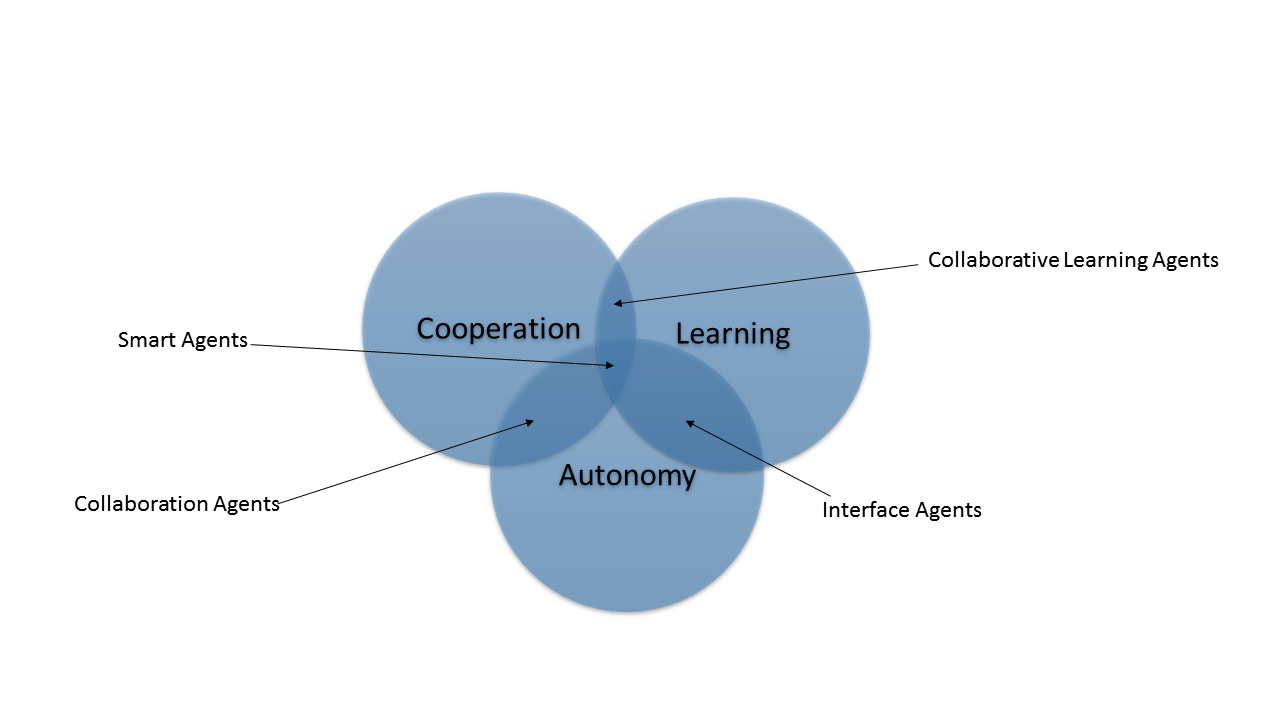
\includegraphics[width=\textwidth]{Figures/agents.png}
	\caption{Dr. Nwana's three primary attributes of agents (Dept. of IECS, Feng Chua University, R.O.C., 2003.)}
\end{figure}

In a study at MIT, Mr. Timothy Bickmore and his partner, Ms. Justine Cassell proposed an interesting model to build trust between users and computer agents \cite{bickmore2001relational}. Provided that in humans, trust is established and maintained by various social interactions such as small talk, Mr. Bickmore and Ms. Cassell argued that the same mechanism can also be used for computer agents to establish trust between users, and them. As an experiment, a computer agent called `REA' was used to communicate with users by performing small talk. REA was able to track the user's movements, and detect their emotional response. The experiment in this study yielded interesting results. It was discovered that users communicating with the REA system using small talk, who also happened to have extrovert personalities, had developed more trust than other users who had more introvert personality traits.

Mr. Bickmore's study indicates that the personality of users can potentially impact the level of trust between humans and agents. An older study conducted on the business school students in California State University yielded similar results. It was discovered that the level of self-esteem in human subjects plays a significant role in their performance and their interaction with a `human-like' computer: ``persons high in self-esteem generated more negative cognitive responses and made fewer errors when faced with human-like rather than machine-like feedback from a computer.'' \cite{resnik1985influence}

A study at University College London titled `Supporting Trust in Virtual Communities' proposes a reputation based trust model designed for improving trust in virtual communities. This trust model is based on `sociological characteristics of trust', such as past experiences and reputation, or `word of mouth'. This proposed model enables agents to take another agent's opinions and recommendations into consideration: ``Our
proposed model allows agents to decide which other
agents’ opinions they trust more and allows agents to
progressively tune their understanding of another agent’s
subjective recommendations.''  Mr. Abdul-Rahman and his colleague, Mr. Hailes argue that although this trust model is designed for increasing trust between humans and virtual societies, this trust model can also be implemented for artificial autonomous agents, and `artificial societies' \cite{abdul2000supporting}.


\subsubsection{Information Security}
At the The Norwegian University of Science and Technology, Mr. Audun Josang published a paper that aimed to focus on the concept of `trust' in the context of information security, and shed some light on the complex nature of Trust. He also examined various types of trust, and trust driven relationships that are relevant in the context of information security, and distributed systems. Mr. Josang provides an interesting definition of trust by defining it from a malicious point of view. He explains that essentially, trust occurs due to the tendency of humans to avoid malicious behaviors of agents (Other people or software). This concept of trust and detecting malicious behavior is critical in computer security due to potential hackers or agents attempting to penetrate a system. He also explores trust and malicious behavior from a philosophical point of view.


A 2006 study by Florina Almenarez et al. proposed a model for managing trust called `Pervasive Trust Management (PTM)' \cite{almenarez2006developing}. `Pervasive' devices are devices which are cumputing at all times. Apple Watches, smart-phones, PDAs etc. are examples of pervasive devices, which have microprocessors that compute things at all times in any network. The increased popularity of such devices produces the issue of trust between these devices communicating with each other, or providing a trusted, secure connection with any network. In this study, Ms. Almenarez, and her colleagues provide a statistical and mathematical trust model to tackle this problem.
\newpage
\subsection{Trust in Networks of Autonomous Systems}
\subsubsection{Multi-Agent Systems}
Chung-Wei Hang and colleagues provide an `adaptive' probabilistic trust model that aims to improve the trust between autonomous agents when they interact with each other in their 2008 paper \cite{hang2008adaptive}. This probabilistic model extends a pre-existing model called W\&S, which is primarily based on a function called PCDF (probability-certainty density
function). In his proposed model, Mr. Hang provides an architecture in which autonomous agents will determine other agents' value of trust, without having any prior  knowledge of them. We believe this is significant, because many of the trusted proposed trust models for autonomous systems are knowledge based. Mr. Wang, and his colleagues also developed a simulation to test their proposed trust model. Their results show that their model is highly capable of estimating the trust of autonomous agents.

%need more work
`Open Distributed Systems' are described as systems that are composed of multiple autonomous agents that interact with each other based on various rules and protocols. \cite{ramchurn2004trust}. At University of Southampton, Sarvapali Ramchurn, Dong Huynh, and Nicholas Jennings have provided a comprehensive study on the currently available trust models in the context of Multi-Agent systems \cite{ramchurn2004trust}. They argue that most of these trust models have one fundamental goal in common: They all aim to minimize the `uncertainty' in the interactions between agents. This study claims that currently, agents have some limitations in their capabilities due to limits in their computations and their storage devices. Thus, when interacting with other agents, or when deciding to do something, they will have a high degree of uncertainty. In `Open distributed systems', agent would have to trust each other in order to reduce this uncertainty in their interactions.

Mr. Ramchurn and his colleagues have analyzed the trust between agents at two levels: the individual level, and system level. At the individual level, various trust models, and evolutionary models are described that help agents in Multi-Agent systems to choose their partners, and interact with them. They can also analyze their interaction with other agents to determine if they are being honest or not. At the system level, this study describes how a Multi-Agent system could be designed to enforce trustworthiness to all agents involved. An example related to agents being involved in an auction was discussed, where the increased trust in agents led to more secure bids and transactions. It was demonstrated that fear of punishment could also be an effective method: ``the threat of future punishment (through
avoidance of or constraining interaction(s)) could be used by reputation mechanisms to prevent
agents from lying about their preferences or forcing them to behave well in an open environment''
\newpage
\begin{figure}
	\centering
		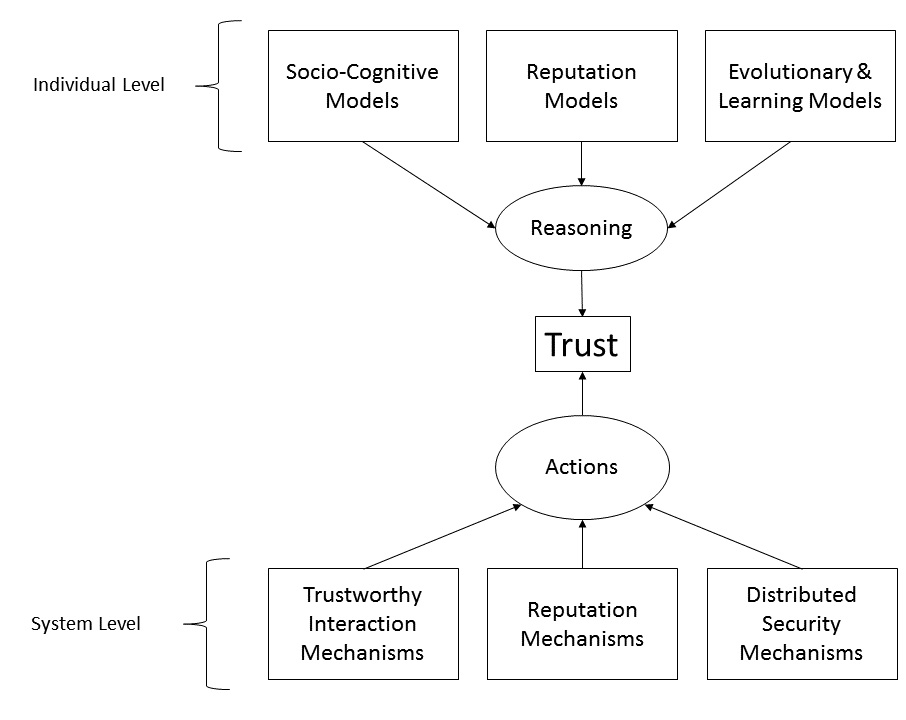
\includegraphics[width=\textwidth]{Figures/MultiAgents.jpg}
	\caption{Trust in Multi-Agent systems \cite{ramchurn2004trust}}
\end{figure}

In 2009, Chung-Wei Hang et al. provided an 'Algebraic' method called 'CertProp' that aims to propagate trust between agents in Multi-Agent systems \cite{hang2009operators}. CertProp uses mathematical functions and operators such as concatenation, aggregation, and selection, in order to propagate trust between the agents. The approach that is used in this study is evidence-based, therefore, the efficiency of this approach has been proven by the evaluation of two data sets.


\subsubsection{Security in Multi-Agent Networks}
In an article, H. Chi Wong and Katia Sycara discuss trust and security in multi-agent systems \cite{wong2000adding}. Given the fact that when in large, open systems, agents interact with other agents that they don't know, the issue of trustworthiness and security arises in these systems. This study proposes a security mechanism that could be used in such systems to enhance security and trust, and address the issues that are currently present in multi-agent systems. The paper provides methods for securing communication between agents, naming methods, and other agent services. Regarding trust between agents, it has been proposed that if entities that deploy agents become responsible for the actions of their agents, the trustworthiness of the agents will increase. Additionally, when agents are communicating, they will have to provide evidence that ``They know secrets that only their delegators know.''


In a paper, Yosi Mass and Onn Shehory investigated distributed trust in open Multi-Agent systems such as online trading systems \cite{mass2001distributed}. They provide a new method in their study that enables agents in a Multi-Agent open system to establish trust between each other, and automatically update this trust overtime. This trust mechanism mainly utilizes `certificates' (Asymmetric Key Exchange) in order to establish trust between agents. This paper claims that this method is efficient, and it can be easily implemented in multi-agent systems.

One paper proposed an algorithm that could be used for agents in multi-agent systems \cite{barber2001belief}. This algorithm enables the agents to analyze the incoming information from various data sources, and distinguish the reliable and trustworthy information from false, deceitful information. This algorithm uses belief systems (Bayesian Networks), which allows the agents to form beliefs based on the trust and reputation of retrieved information, and revise them overtime. This study conducted two experiments, one in static multi-agent environments, and the other in dynamic environments. The results of these experiments indicate that in static environments, this algorithm performs efficiently. In dynamic systems however, there were some delays for the agents to process and revise their Bayesian beliefs.

Another paper by Trung Dong Huynh and colleagues introduced a trust and reputation model called `FIRE' \cite{huynh2006integrated}. This model could be used in open multi-agent systems to measure the performance of agents in the systems. FIRE takes into account several factors: ``FIRE incorporates interaction trust,
role-based trust, witness reputation, and certified reputation to provide trust metrics in most
circumstances''. Additionally, this study introduced a framework that aims to collect meta-data from various sources such as past interactions, witnesses, and rules about the environment for measuring the agent trust. This model allows the agents to choose their partners carefully by evaluating the trust measures they have access to. This improves the overall performance of agents in multi-agent systems.

Stefan Poslad and Monique Calisti investigated trust and security in FIPA agents, and discuss its strengths and weaknesses \cite{poslad2000towards}. FIPA, which stands for `Foundation for Intelligent Physical Agents' is a non-profit organization that was created in 1996 to produce a series of standard specifications for the development of intelligent agents in multi-agent systems. In FIPA, there are two main concepts that are discussed in this paper: agents, and agencies. FIPA agencies are described as the environment in which agents are present. They provide the agents a series with support services called `Middle-Ware Services', which grant them the capability of interacting with other agents within the same agency, or agents from other agencies. There are two types of Middle-Ware Services: AMS (Agent management system), and DF (directory facilitator). This study examines the trust between various entities in a FIPA system. The trust model in FIPA consists of trust between agents and AMS, trust between service providers and DF, trust between service user agents and DF, and trust between agents and the `Agent Communication Chanel'. 

This study concludes that the current trust models used in FIPA systems are not optimal. As a result, it is easy for malicious agents or hackers to take advantage of service providers in order to manipulate the agents, or attack the system. Additionally, it was discovered that the current security systems related to FIPA are not effective at all, and are obsolete by today's standards.


Piotr Gmytrasiewicz and Edmunt Durfee investigated trust and honesty between fully automated autonomous agents \cite{gmytrasiewicz1993toward}. In their paper, `Toward a Theory of Honesty and Trust Among
Communicating Autonomous Agents', they provided a method that could be used to improve communication between agents. This recursive method allows autonomous agents to calculate the outcomes of their messages before sending them to other agents. Analysis in this study indicated that although in some cases, agents might conclude the messages they are about to send might not be believable on the receiving side, communication occurs between the agents regardless. In some cases however, it was discovered that it is possible that some agents stop believing what they are told by other agents, which reduces the effectiveness of communication between them.


Y.C. Jiang et al. present a model for constructing trust between agents in multi-agent systems \cite{jiang2005autonomous}. This `Autonomous Trust Construction' model utilizes graph searches that allows the agents to build trust effectively. This study introduces the concepts of `Path Searching' and `Trust Negotiation'. Path Searching uses a graph search to find a `Trust Path'. It is proposed that if an agent cannot find the Trust Path by performing a graph search, it can proceed to automatically `negotiate trust' with the other agent, which mainly deals with exchanging sensitive data. The experimental results of the simulations in this study indicates that this trust construction model is highly effective.

\begin{figure}
	\centering
		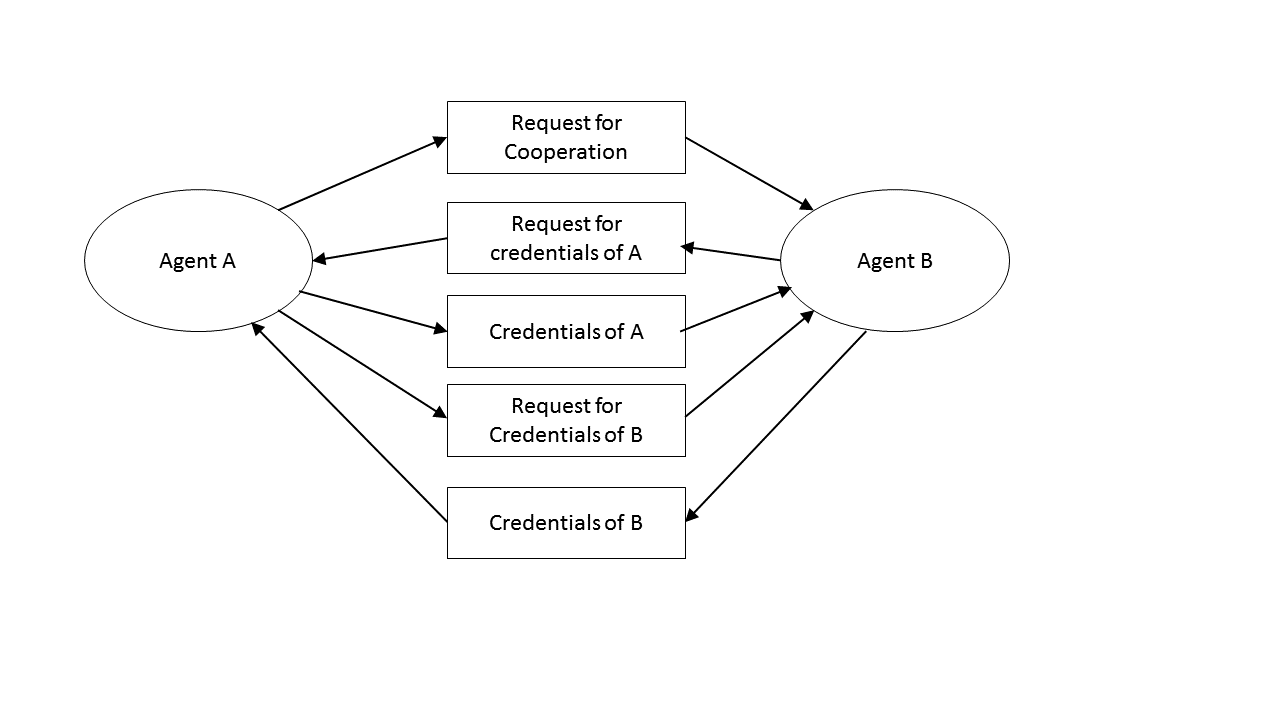
\includegraphics[width=\textwidth]{Figures/TrustNegotiation.png}
	\caption{Trust Negotiation example in \cite{jiang2005autonomous}}
\end{figure}


\subsubsection{Wireless Networks}
Wireless communications is one of the fields that has been growing very fast in the recent years. Due to increased complexity and use of wireless communication methods such as `pervasive devices', mobile networks, and P2P networks, the need for ensuring trust and reliability in these systems arises. Mr. Tao Jiang and his research partner, John Baras provided a case study on Distributed Trust Management \cite{jiang2006trust}. They introduced a statistical trust evaluation to evaluate and measure trust in agents involved in a network. Then, they provided a mathematical proof that proved that their trust evaluation method works, and affects the level of performance.

\subsubsection{Social Networks}
Frank Walter and his colleagues argue that due to the exponential boom of the internet in the recent years, the amount of information available to uses has been increased significantly, causing `information overload' for users \cite{walter2008model}. Thus, there might be a need for a system that can filter the available information based on the needs of the user. As a solution, they introduced a trust-based recommendation system to be used in social networks. In this model, agents can filter the amount of information given to them based on the level of trustworthiness of other agents. They also use their social network to retrieve information that is unknown to them. Based on a series of experiments and simulations, this study indicates that the performance of this recommendation system is satisfactory.

In another similar study on trust between agents in social networks, Stefano Battiston and coworkers \cite{battiston2006impact} provided an `Automated Distributed Recommendation
System' that could be implemented on agents in social networks. In this proposed model, agents use their social network in order to construct a query to conduct a search. Furthermore, it has been stated that based on the preferences of agents, the trust between the other `neighbor' agents and the main agent could be used to filter the search result. The computer simulations in this study indicate that the `heterogeneity' of preferences in agents in a social network plays a major role on the impact of trust on the performance of the recommendation system. It was discovered that if the agents have mild heterogeneous preferences, trust between agents positively impacts the performance of the system, as opposed to agents with higher levels of heterogeneity in their preferences.

In a study, Josep Pujol and colleagues proposed a method called NodeRanking, which could be used to extract reputation in multi-agent systems by using `social network topology' \cite{pujol2002extracting}. This method is based on the idea that the position of each agent within the social network could be used in order to calculate the amount of reputation. This study also conducts an experiment on a live social network community to test its method. The paper claims that its proposed method is superior compared to other reputation extracting methods because it doesn't rely on users providing ratings (feedback) as an input.

\subsubsection{P2P Networks}
A study by Yao Wang and Julita Vassileva proposed a `Bayesian' networked-based trust model that could be used in P2P (peer to peer) networks \cite{wang2003bayesian}. This study argues that in an open P2P network, there might be malicious, or defective agents (nodes) present in the system. This is due to the fact that in an open P2P system, there is no authority and as a result, methods of acquiring trust and reputation could be used in this systems to distinguish good peers from bad and malicious ones. This study considers a P2P file sharing system in order to explain the Bayesian method mentioned earlier. In file sharing P2P systems, there are `seeders' (or File Provides) and `peers' (File receivers, or agents). In this provided example, agents usually care about download speeds, file quality, and file type. Thus, agents are capable of developing a `Bayesian' network for seeders that they have interacted with. The values of 1 and 0 are used for displaying the level of satisfaction of the agents.

\begin{figure}
	\centering
		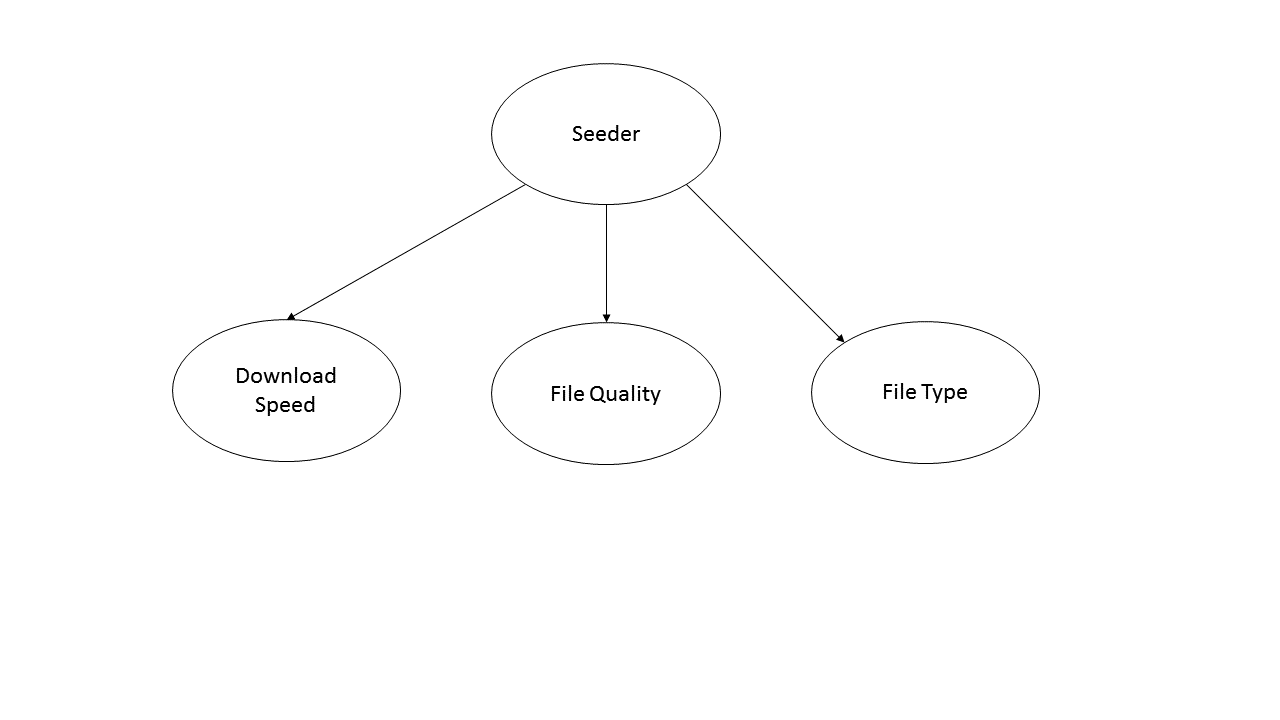
\includegraphics[width=\textwidth]{Figures/p2pTrust.png}
	\caption{Qualities that increase satisfaction in a P2P Bayesian Network}
\end{figure}

The Yang-Vassileva study tested this Bayesian trust model by simulating a file sharing P2P network, and the results indicate that agents that communicate their recommendations to each other have high performance, as opposed to agents that don't communicate as much. Ms. Wang and Ms. Vassileva claim that this approach can also be used in other areas.


\section{Summary}

\begin{center}
	

\begin{tabular}{ |p{2cm}|p{4cm}|p{6cm}|  }
\hline
\multicolumn{3}{|c|}{List of Studies} \\
\hline
Category & Year/Researcher/Study & Results \\
\hline
Humans-Robots & 2008 D. Stormont - `Analyzing Human Trust of Autonomous Systems in Hazardous Environments' & Confidence plays an important role as well as trust\\
 & & The unpredictability of the robot affects trust \\
\hline
 & 2001 B. Esfandiari, S. Chandrasekharan - `On How Agents Make Friends: Mechanisms for Trust Acquisition' & Mathematical definition for trust, where trust is a variable T\\
 & & Trust acquisition is the process or mechanism that allows the calculation and update of 'T' \\
\hline
& 2011 P. Hancock et al. - `A Meta-Analysis of Factors Affecting Trust in Human-Robot Interaction' & the performance of the robot has the biggest impact on trust in the context of HRI\\
\hline
& 2013 J. Penders et al. - `Enhancing Trust and Confidence in Human Robot Interaction' &  \\
\hline
& 2008 S. Merritt - `Not All Trust Is Created Equal: Dispositional and History-Based Trust in Human-Automation Interactions' & Different people have different levels of trust toward robot despite its constancy\\
\hline
& 2004 R. Parasuraman, C. Miller - `Trust and Etiquette in High-Criticality Automated Systems' & Etiquette affects human trust and the reliablity of autonomous robots\\
\hline
& 2012 R. Yagoda, D. Gillan - `You Want Me to Trust a Robot? The Development of a Human-Robot Interaction Trust Scale' & Created the HRI `Trust Measuring Tool'\\
\hline
& 2014 Y. Wang et al. - `Human-robot Mutual Trust in (Semi) Autonomous Underwater Robots' & If the human trusts the robot, its performance increases\\
\hline
Humans-Self Driving Cars & 2013 D. Howard - `Public Perceptions of Self-Driving Cars: The Case of Berkeley, California' & most consumers like SDC's\\
 & & Different people have different trust issues\\
\hline
& 2014 M. Carlson - `Identifying Factors That Influence Trust in Automated Cars and Medical Diagnosis Systems' & Most people tend to prioritize safety, accuracy, and failure rates when trusting an autonomous system\\
\hline
\end{tabular}

\begin{tabular}{ |p{2cm}|p{4cm}|p{6cm}|  }
\hline
\multicolumn{3}{|c|}{List of Studies} \\
\hline
 & 2015 M. Kyriakidis et al. - `Public Opinion on Automated Driving: Results of an International Questionnaire Among 5000 Respondents' & The geographic positioning and education of consumers affects the premises of their trust\\
\hline
 & 2015 M. Wagner, P. Koopman - `A Philosophy for Developing Trust in Self-Driving Cars' & Users testing; relying and improving will increase their trust in the robot\\
\hline
 & 2013 T. Helldin - `Presenting System Uncertatinty in Automative UIs for Supporting Trust Calibration in Autonomous Driving' & If people know about the problems of a robot, they will probably override it to avoid them\\
\hline
Human-Autopilot Modes & 2015 S. Winter et al. - `Indian and American Consumer Perceptions of Cockpit Configuration Policy' & Culture affects trust\\
\hline
 & 2015 V. Bukatov P. Ioannou - `Driving Autopilot With Personalization Feature for Improved Safety and Comfort' & People have an easier time trusting familiar things.\\
\hline
Human-Agents (Software Agents) & 2003 Nwana - `Software Agents: An Overview' & Agents have secondary attributes that affect trust\\
\hline
 & 2001 T. Bickmore, J. Cassell - `Relational Agents: A Model and Implementation of Building User Trust' & Small talk builds trust, especially with extroverted personalities\\
 & & The personality of users can impact the level of trust between humans and robots\\
\hline
 & 2000 Abdulrahman, Hailes - `Supporting Trust in Virtual Communities' & Model designed to increase trust between agents and agents, and humans and agents\\
\hline
Information Security & A. Josang & Trust occurs due to the tendency of humans to avoid malicious behaviors of agents\\
\hline
 & 2006 F. Almenarez et al. - `Developing a Model for Trust Management in Pervasive Devices' & Mathematical trust model designed to tackle the issue of trust between agents, creating secure connections etc.\\
\hline
Multi-Agent Systems & 2008 C. Hang et al. - `An Adaptive Probabilistic Trust Model and Its Evaluation' & Model that improves trust between autonomous agents when they interact with one another\\
\hline
 & 2004 S. Ramchurn, D. Huynh, N. Jennings - `Trust in Multi-Agent Systems' & Agents have limitations in their capabilities, so they have a high degree of uncertainty when dealing with other agents\\
\hline
\end{tabular}

\begin{tabular}{ |p{2cm}|p{4cm}|p{6cm}|  }
\hline
\multicolumn{3}{|c|}{List of Studies} \\
\hline
 & 2009 C. Hang et al. - `Operators for Propagating Trust and Their Evaluation in Social Networks' & Introduces CertProp; propogates trust between agents\\
\hline
Security in Multi-Agent Systems & 2000 H. C. Wong, K. Sycara -`Adding Security and Trust to Multi-Agent Systems' & Proposes methods for securing communication between agents\\
\hline
 & 2001 Barber - `Belief Revision Process Based on Trust: Simulation Experiments' & Propose algorithm that enables agents to tell if incoming data is trustworthy or false\\
\hline
 & 2001 Y. Mass, O. Shehory - `Distributed Trust in Open Multi-Agent Systems' & Provides a new method that enables agents in a multi-agent open system to establish trust between each other and automatically update the trust over time\\
\hline
 & 2000 S.Poslad, M. Calisti - `Towards Improved Trust and Secutiry in FIPA Agent Platforms' & FIPA trust methods are not optimal and are obsolete by today's standards\\
\hline
 & 1993 P. Gmytrasiewicz, E. Durfee - `Toward a Theory of Honesty and Trust Among Communicating Autonomous Agents' & Provides method that improves communication between agents\\
\hline
 & 2005 Y. C. Jiang et al. - `Autonomous Trust Construction in Multi-Agent Systems Graph Theory Methodology' & Presents a model for constructing trust in multi-agent systems\\
\hline
Wireless Networks & 2006 T. Jiang J. S. Baras - `Trust Evaluation in Anarchy: A Case Study on Autonomous Networks' & Introduces a statistical trust evaluation to evaluate and measure trust in agents involved in a network\\
\hline
Social Networks & 2006 F. Walter et al. - `Impact of Trust on the Performance of a Recommendation System ' & Introduces a trust-based system in which agents can filter the amount of information given to them\\
\hline
 & 2008 S. Battiston et al. - `A Model of a Trust-based Recommendation System on a Social Network' & Proposes a model where agents use their social network in order to construct a query to conduct a search\\
\hline
 & 2002 J. Pujol et al. - `Extracting Reputation in Multi-Agent Systems by Means of Social Network Topology' & proposes a method which can be used to extract reputation in multi-agent systems\\
\hline
P2P Networks & Y. Wang, J. Vassileva - `Bayesian Network Trust Model in Peer-to-Peer Networks' & Proposes a Bayesian trust model that could be used in P2P networks\\
\hline
\end{tabular}

\end{center}


%\begin{table}[]
%\centering
%\caption{My caption}
%\label{my-label}
\begin{longtable}{|c|c|p{5cm}|p{3cm}|p{1cm}|}
\hline
\multicolumn{5}{|c|}{List of Studies}                                                                                               \\ \hline
Category                        & Study & \multicolumn{1}{c|}{Summary}    & \multicolumn{1}{c|}{Technology} & \multicolumn{1}{c|}{} \\ \hline
\multirow{8}{*}{Human - Robots} 
	& \cite{stormont2008analyzing}    
	&  Confidence plays an important role as well as trust, and The unpredictability of the robot affects trust  
	& Tech                            
	&                       
	\\ \cline{2-5} 
	& \cite{esfandiari2001agents}     
	& Mathematical definition for trust, where trust is a variable T. Trust acquisition is the process or mechanism that allows the calculation and update of 'T'
	&                                 
	&                       
	\\ \cline{2-5} 
	&    
	& 
	&                                 
	&
	\\ \cline{2-5}
	&    
	& 
	&                                 
	&
	\\ \cline{2-5} 
	&    
	& 
	&                                 
	&
	\\ \cline{2-5} 
	&    
	& 
	&                                 
	&
	\\ \cline{2-5} 
	&    
	& 
	&                                 
	&
	\\ \cline{2-5} 
	&    
	& 
	&                                 
	&           
	\\ \hline
\multirow{5}{*}{Human SDC}      
	& 5     
	& text                            
	&                                 
	&                       
	\\ \cline{2-5} 
	& 5     
	& text                            
	&                                 
	&                       
	\\ \cline{2-5} 
	& 5     
	& text                            
	&                                 
	&                       
	\\ \cline{2-5} 
	& 5     
	& text                            
	&                                 
	&                       
	\\ \cline{2-5} 
	& 7     
	& test                            
	&                                 
	&                       
	\\ \hline
	
	\multirow{2}{*}{Human-Autopilot Modes}    
	& 5     
	& text                            
	&                                 
	&                       
	\\ \cline{2-5} 
	& 7     
	& test                            
	&                                 
	&                       
	\\ \hline
	
	\multirow{3}{*}{Human-Agents (Software) } 
	& 5     
	& text                            
	&                                 
	&                       
	\\ \cline{2-5}
	& 5     
	& text                            
	&                                 
	&                       
	\\ \cline{2-5} 
	& 7     
	& test                            
	&                                 
	&                       
	\\ \hline
	
	\multirow{2}{*}{Information Security } 
	& 5     
	& text                            
	&                                 
	&                       
	\\ \cline{2-5} 
	& 7     
	& test                            
	&                                 
	&                       
	\\ \hline
	
	\multirow{3}{*}{Multi-Agent Systems }
	& 5     
	& text                            
	&                                 
	&                       
	\\ \cline{2-5}
	& 5     
	& text                            
	&                                 
	&                       
	\\ \cline{2-5} 
	& 7     
	& test                            
	&                                 
	&                       
	\\ \hline
	\multirow{6}{*}{Security in Multi-Agent System}
	& 5     
	& text                            
	&                                 
	&                       
	\\ \cline{2-5} 
	& 5     
	& text                            
	&                                 
	&                       
	\\ \cline{2-5}
	& 5     
	& text                            
	&                                 
	&                       
	\\ \cline{2-5} 
	& 5     
	& text                            
	&                                 
	&                       
	\\ \cline{2-5}
	& 5     
	& text                            
	&                                 
	&                       
	\\ \cline{2-5} 
	& 7     
	& test                            
	&                                 
	&                       
	\\ \hline
	
	\multirow{1}{*}{Wireless Networks}
	& 7     
	& test                            
	&                                 
	&                       
	\\ \hline
	
	\multirow{3}{*}{Social Networks}
	& 5     
	& text                            
	&                                 
	&                       
	\\ \cline{2-5}
	& 5     
	& text                            
	&                                 
	&                       
	\\ \cline{2-5} 
	& 7     
	& test                            
	&                                 
	&                       
	\\ \hline
	
	\multirow{1}{*}{P2P Networks}
	& 7     
	& test                            
	&                                 
	&                       
	\\ \hline
%\end{tabular}
\end{longtable}

\section{Open Problems, Future Directions and Concluding remarks}
%\bibliographystyle{abbrv}
\bibliography{ShervinTrustSurvey}

\end{document}
